\documentclass{beamer}
\setbeamertemplate{navigation symbols}{}
\setbeamertemplate{itemize item}[ball]
\setbeamertemplate{itemize subitem}[circle]

\usepackage{pgfpages}
\pgfpagesuselayout{4 on 1}[a4paper,border shrink=5mm]

\title{Seri}
\subtitle{A High-Level User Language for SMT Queries}
\author{Richard Uhler}

\begin{document}

\begin{frame}
    \titlepage
\end{frame}

\begin{frame}{How to Implement a Sudoku Solver}
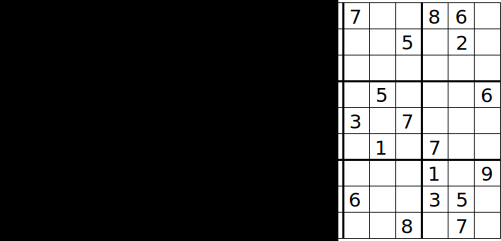
\includegraphics[width=\textwidth]{input2}
\end{frame}

\begin{frame}{How to Implement a Sudoku Solver}
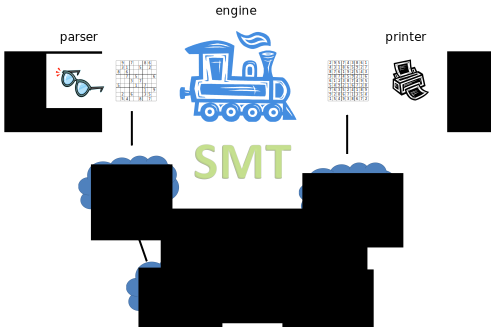
\includegraphics[width=\textwidth]{current8}
\end{frame}

\begin{frame}{How to Implement a Sudoku Solver}
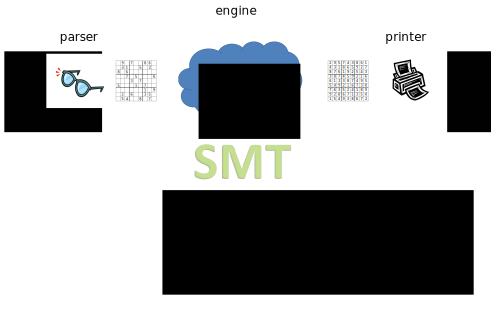
\includegraphics[width=\textwidth]{current11}
\end{frame}
 
\begin{frame}{The Parser in Seri}
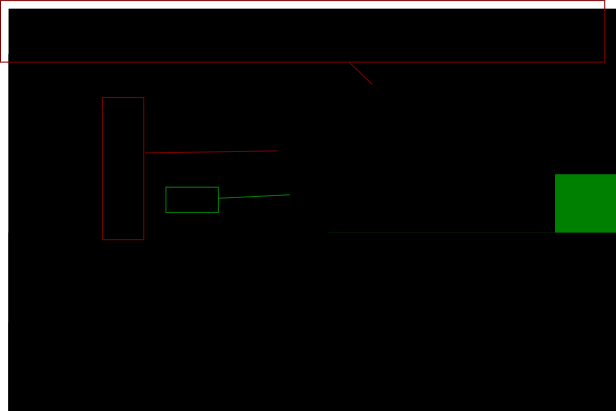
\includegraphics[width=\textwidth]{parser8}
\end{frame}

\begin{frame}{The Sudoku Constraints}
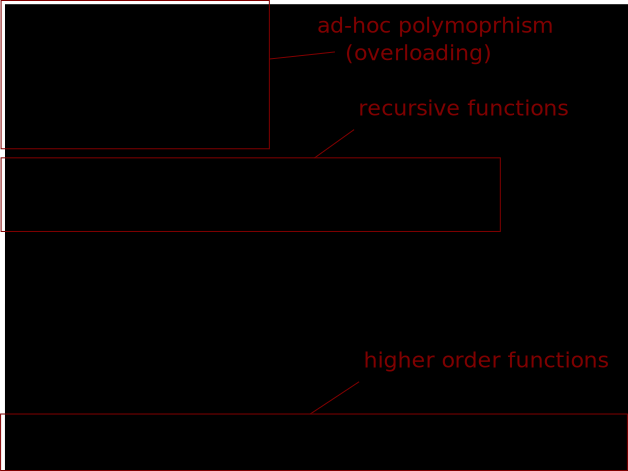
\includegraphics[width=\textwidth]{isvalid10}
\end{frame}

\begin{frame}{The Sudoku Solver}

\includegraphics[width=0.9\textwidth]{main3}
\begin{itemize}
\item Yices1: 1m15s
\item Yices2: 1.6s
\end{itemize}
\alert{No change in source code going from Yices1 to Yices2!}
\end{frame}

\begin{frame}{A Different Cell Representation}

\includegraphics[width=0.7\textwidth]{bitcell7}
\begin{itemize}
\item Yices1: 3m53s (was 1m15s)
\item Yices2: 1.0s  (was 1.6s)
\end{itemize}
\end{frame}

\begin{frame}{Interactive and Reusable Queries}

\includegraphics[width=0.8\textwidth]{allq4}
\end{frame}

\begin{frame}{Current Status, Future Plans}
\begin{block}{Current Status}
    \begin{itemize}
        \item Yices1, Yices2 supported
        \item All queries shown work
    \end{itemize}
\end{block}
\begin{block}{Future Work (Ph.D. Thesis)}
    \begin{itemize}
        \item Optimize generated queries
        \item Add support for more solvers
        \item Integrate tool more seamlessly with Haskell
        \item Explore implementation of formal tools, such as model checkers,
              built in Seri with reusable library components
    \end{itemize}
\end{block}
\end{frame}

\end{document}

